\documentclass[a4paper,12pt]{article}

\usepackage[utf8]{inputenc}
\usepackage[a4paper, total={6in, 9in}]{geometry}
\usepackage{listings}
\usepackage{lstautogobble}
\usepackage{color}
\usepackage{amssymb}
\usepackage[parfill]{parskip}
\usepackage{pgfplots}
\usepackage{tikz}
\usepackage{pgfgantt}
\usepackage{adjustbox}
\usepackage{graphicx}
\usepackage{pdfpages}
\usepgfplotslibrary{groupplots}
\pgfplotsset{width=6.9cm,compat=1.9}

\begin{document}
	%\nocite{*}
	% Title page
	\begin{titlepage}
	
		\centering
	
		{\large \scshape Electronics and Computer Science \par}
		{\large \scshape Faculty of Physical Sciences and Engineering \par}
		{\large \scshape University of Southampton \par}
		\vspace{3cm}
		
		{\Large \textbf{Martin Valchev} \par} % Put your name here
		\vspace{0.25cm}
		{\large \today \par}
		
		\vfill
		
		\hrule height 0.4pt
		\vspace{1cm}
			\huge
			\textbf{Analysis and Application of Active Learning to Classify Malicious Twitter Posts} % Put your project title here
		\vspace{1cm}
		\hrule height 1.2pt
		
		\vfill
		
		{\Large Project supervisor: \\ Oliver Bills \par} % Put your supervisor here
		\vspace{0.5cm}
		%%{\Large \textit{Second examiner}: \\ Caesar Anthonio Zeppeli \par} % Put your second supervisor here
	
		\vfill
		
		{\Large A project progress report submitted for the award of \par} % Change this depending on final / progress / brief
		{\LARGE BEng Software Engineering \par} % Put your degree title here
		\vspace{4cm}
	
	\end{titlepage}

\section*{Abstract}
With social media being crucial for maintaining social status now more than ever, the notion of ``cancel culture" has become increasingly prevalent. Malicious people aim to ``cancel" or deplatform others in the form of cyberbullying.

To combat this problem, a common approach is to apply supervised machine learning on large labeled datasets. However, while unlabeled data can often be obtained trivially, labeled one is much more scarce. Moreover, labeling such textual data is expensive and time-consuming, as that is usually done manually by humans.

This project explores active learning as an alternative, more data-efficient approach, and reviews its efficacy in the context of cyberbullying detection, compared to various machine learning techniques. Specifically, it aims to show how applying activate learning in the domain of Natural Language Processing can reduce data labeling costs and improve data efficiency, while maintaining high classification accuracy.
\section*{Scope}
While the methods and outcomes of this project could be generalised to all social media, this project focuses on Twitter specifically. The project does not necessarily aim to produce a highly accurate model for post classification, but rather show data cost in relation to $f_1$-score of models trained using various machine learning techniques.
%%\newpage
\section*{Project Goals}
\begin{itemize}
    \item To compile an appropriate data set for machine learning using Twitter's API, feature selection and feature engineering.
    \item To build an application that interactively queries the user to label data.
    \item To apply active learning to train a model for classifying Twitter posts.
    \item To produce an in-depth analysis of the characteristics and outcomes of applying active learning.
    \item To compare active learning to other machine learning approaches in regards to data efficiency. 
\end{itemize}
\newpage
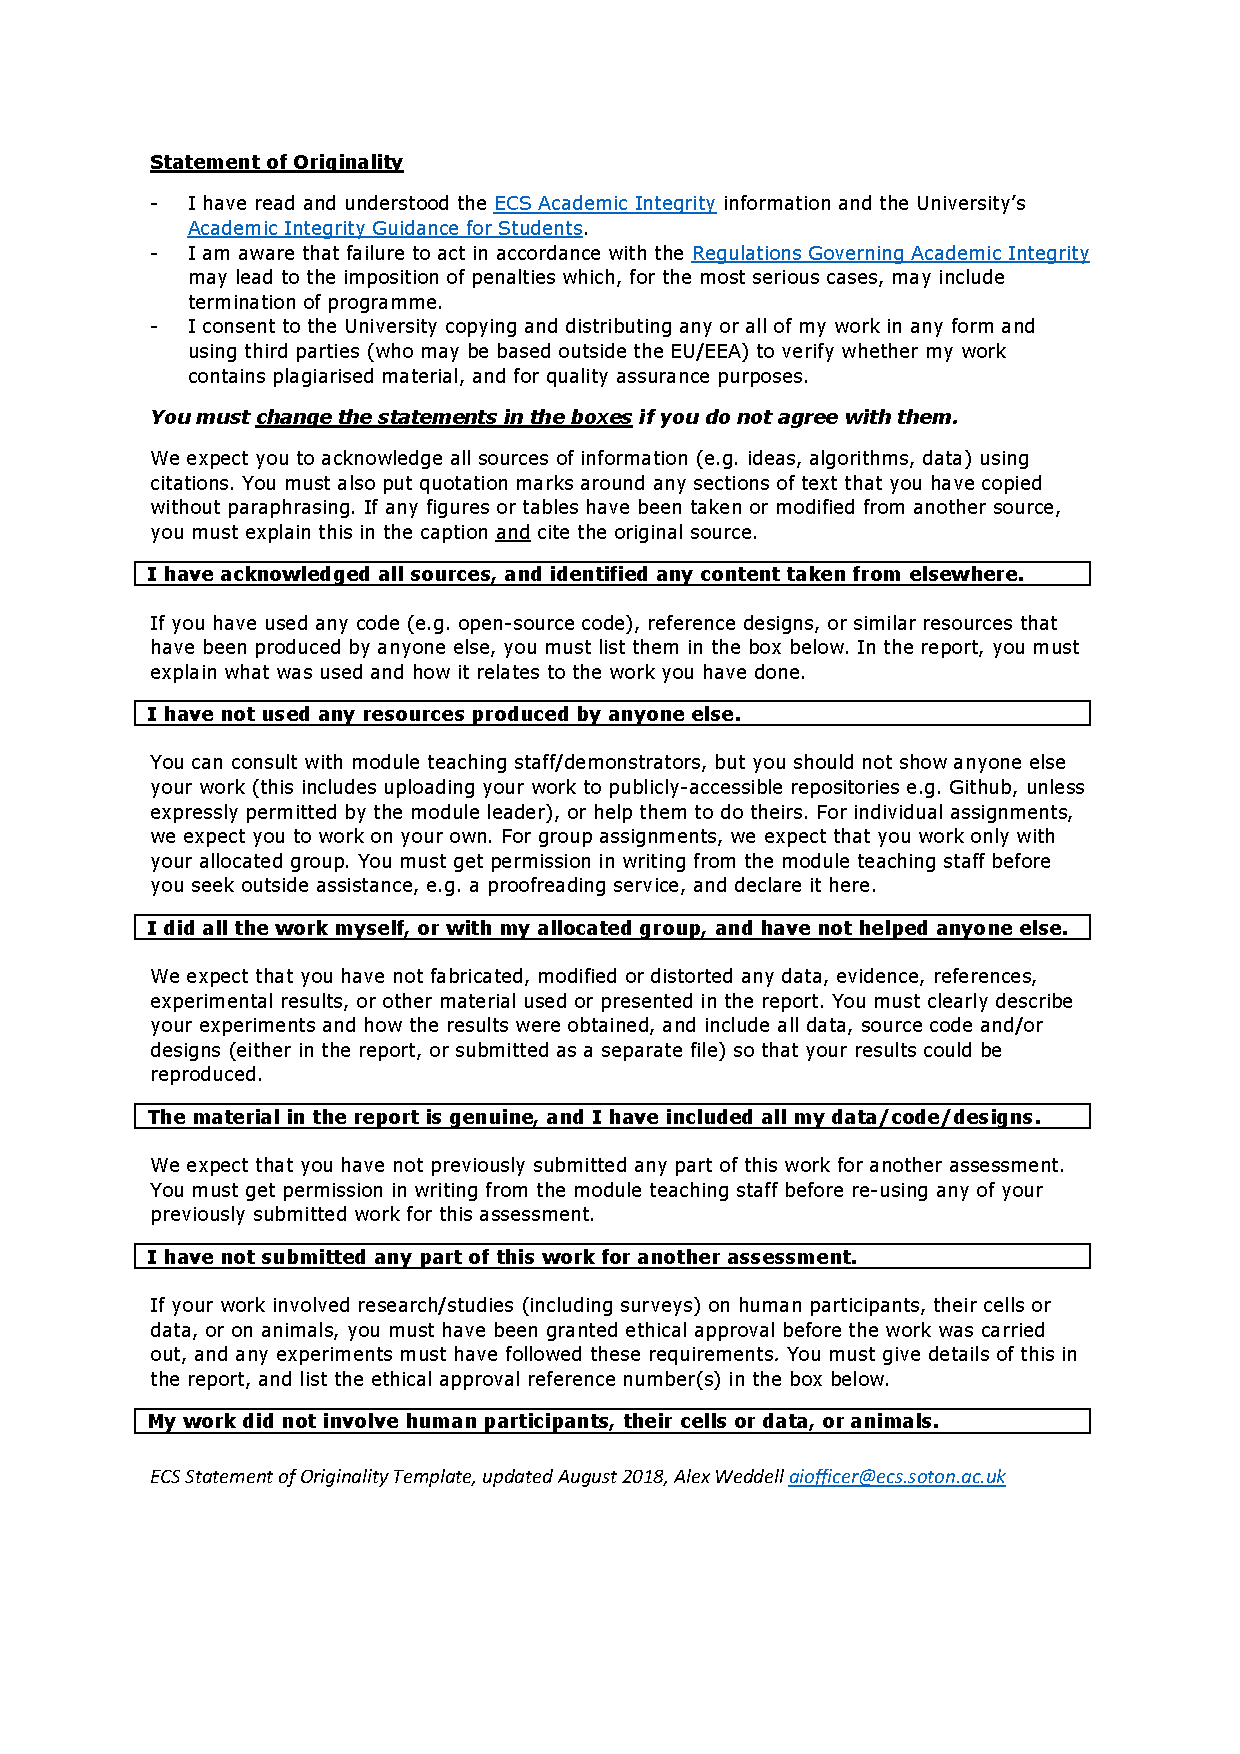
\includepdf[pages={1},pagecommand={},scale={0.9}]{ai_statement.pdf}
\tableofcontents
\newpage
\section{Introduction}
%It is the technique of collaborative learning, where the machine asks an "oracle" to label only data that it deems most beneficial for improving the model in its current state, based on various sampling strategies.
Active Learning is a special case of machine learning in which a learning algorithm can interactively query a user, sometimes referred to as an ``oracle", to label previously unseen data points, or those that the model is least confident about.

``The key idea is that an algorithm can achieve greater accuracy with fewer labeled training instances if it is allowed to choose the training data from which is learns."\cite{Settles2009}

There are a few core design decisions that are to be made when implementing active learning. The following section reviews them, as well as different approaches regarding machine learning and cyberbullying detection, evaluates their pros and cons, and draws conclusions about their applicability to the project.
%%\newpage
\section{Literature Review}
It is important to note, that a lack of consistency in dataset and evaluation process between different literature makes direct comparison of their findings impossible.
\subsection{Feature Selection and Feature Engineering}
\subsubsection{User Features}
Dadvar M. et al. \cite{Dadvar2013} propose the use of profile data as features, in addition to NLP for tweets, to further improve the $f_1$-score of cyberbullying classification. That is, to derive the common behaviour of users based on patterns of offensive language in previous posts, average length of the comments, age, number of pronouns, etc. The authors find that including user-based information yields approximately only $6.6\%$ increase to $f_1$-score in their most successful attempt. They conclude that ``users' profile information is not always stated correctly", which attributes to the underwhelming result.

Al-Garadi et al. \cite{garadi-highestf/top10features} perform an analysis over a set of features, including network, activity, user and textual information, to identify which features are most significant and provide the largest information gain in the context of cyberbullying detection. Four out of the top 10 features are user-related, which alludes to user data being a significant part of the $42\%$ AUC increase over their baseline textual features, for a total of $0.943$. While their results are impressive, the difference in performance is marginal compared to other state-of-the-art literature that avoids the use of profile data. Again, due to the lack of consistency in dataset and evaluation process between different literature, it is hard to gauge how beneficial user profile information is, therefore I will collect such data to experiment with during prototyping.

Alternatively, one could opt to predict user behaviour with a separate classifier and use the resulting labels as a categorical feature for training the cyberbullying model. Balakrishnan V. et al. \cite{Balakrishnan2020} are able to classify Twitter users as ``Bully, Aggressor, Spammer and Normal" with an $f_1$-score of $\approx0.91$ by utilising personality and sentiment data. The difference in approach to cyberbullying detection they've taken makes direct comparison not possible, but the results are promising. However, as the increase in data cost required to perform this task goes against my goal to use less labelled data to achieve comparable $f_1$-score, predicting user behaviour will not be taken into consideration for the implementation of this project.
\subsubsection{Textual Features}
Textual features are by far the most commonly used features in cyberbullying classification, likely due to the key role profanity plays in malicious texts.
The following techniques are often used in topical literature to extract textual features:
\begin{itemize}
    \item TF-IDF - measure of word importance in a text
    \item Bag-of-Words - histogram of the words in a text
    \item Named-entity Recognition - named entities mentioned in a text
    \item Sentiment Analysis - emotion/opinion of a text
    \item Word2vec - word embeddings/associations
\end{itemize}
Rosa H. et al. \cite{Rosa2019} suggest that feature engineering beyond the use of pure TF-IDF is not rewarding.
\subsubsection{Other Features}
Research by Al-Garadi et al. \cite{garadi-highestf/top10features} indicates that other types of features can also be utilised successfully, but contribute less to the overall performance of a cyberbullying classification model. These features are less appealing and an unlikely approach for this project. Examples of such features are:
\begin{itemize}
    \item Network Features - number of followers, followed users, following–followers ratio, verification status, etc.
    \item Activity Features - number of posts, mentions, tweets added to favorites, hashtag usage, etc.
\end{itemize}
\subsubsection{Feature Selection}
Feature selection is best analysed by Rosa H. et al. \cite{Rosa2019}, who explore 22 different papers on the topic of automatic cyberbullying detection, as well as perform their own experiment. They found 3 best-performing scenarios/combinations:
\begin{itemize}
    \item TF-IDF (pure)
    \item TF-IDF + Word Embeddings
    \item TF-IDF + Personality Features + Word Embeddings
\end{itemize}
\subsection{Classification Algorithms}
Active learning by definition requires a probabilistic classifier that outputs a confidence measure for its predictions.

Neural networks are known for their inability to produce such measures accurately \cite{Nguyen2015}. They are often overconfident in their labeling, which introduces bias during active learning sampling.
Recent study proposes a novel loss function that can be applied to existing neural network architectures without any modification, which results in reliable predictions and is effective for active learning \cite{Moon2020}. However, implementing a different loss function for a specific algorithm diverges from the idea of minimal variance during the evaluation of this project. Moreover, the novelty of the approach may result in a poor implementation and is therefore a project risk. Neural networks also require much more data to perform well in comparison to traditional machine learning algorithms. As such, neural networks won't be considered.

Precisely because of the importance of accurate confidence measures, naturally probabilistic classification models, i.e. the model predicts a probability distribution over the classes, are more suitable for the active learning task. Examples of such models are Logistic Regression, Naive Bayes, Random Forest, etc. SVM is a notable exception, whose ``convenient mathematical properties" make it ``well-suited for active learning", as discussed by Kremer J. et al. \cite{Kremer2014}.

Active learning for cyberbullying classification hasn't been explored yet in academic literature. The topic of cyberbullying detection itself however has been highly studied. One of the best-performing models has been proposed by Al-Garadi et al. \cite{garadi-highestf/top10features}. In their paper, the performance of four classifiers (NB, LIBSVM, Random Forest and KNN) is measured based on various features. Results suggest that the choice of classifier doesn't impact $f_1$-score as much as the choice of features and dataset balance do. For example, there is only $1.865\%$ difference between their lowest-scoring Naive Bayes approach and their highest-scoring KNN ``under a basic setting". As such, this project will focus on exploring classifiers that are known to perform well in active learning environments, regardless of task, and not necessarily ones that have been shown to work with cyberbullying classification specifically.
\subsection{Active Learning Scenarios}
In the case of Membership Query Synthesis, the model can request labels for both unlabeled data instances from the dataset and ones that are instead generated by the machine \cite{Settles2009}. This is clearly not a good approach for natural language tasks, such as the one of cyberbullying classification. Cyberbullying is not always apparent even in well-structured text and chances are the machine would not be able to generate sensible data that contains bullying traces. Any label given to nonsensical instances may well degrade the performance of the model on actual testing data. There are recent advances in the field of query synthesis for natural language that show promising results \cite{schumann-rehbein-2019-active}, however, more suitable approaches exist.

One such approach is Stream-Based Selective Sampling. Unlabeled data instances are drawn sequentially and the machine decides whether to label each one individually \cite{Settles2009}. This would work well in practice, as one could fetch fresh tweets as a stream from Twitter's API and the machine would decide for each tweet whether it is worth labeling. This is however not applicable to this project because one of the requirements for evaluation is that the dataset must be consistent for all machine learning classifiers, in order to minimise variance.

This leads to the final and most suitable approach - Pool-Based Sampling. In this scenario, data instances are sampled from a pool, consisting of both labeled and unlabeled data, based on some sampling strategy \cite{Settles2009}. This allows for all machine learning classifiers that are to be implemented in this project to share a single dataset.
\subsection{Data Analysis}
The following graphs aim to visualise the relation between dataset size and balance, and $f_1$-score, based on works by Zhao et al. (2016) \cite{Zhao2016}, Singh et al. (2016) \cite{Singh2016}, Zhao and Mao (2016) \cite{Zhao2017} and Al-Garadi et al. (2016) \cite{garadi-highestf/top10features}.

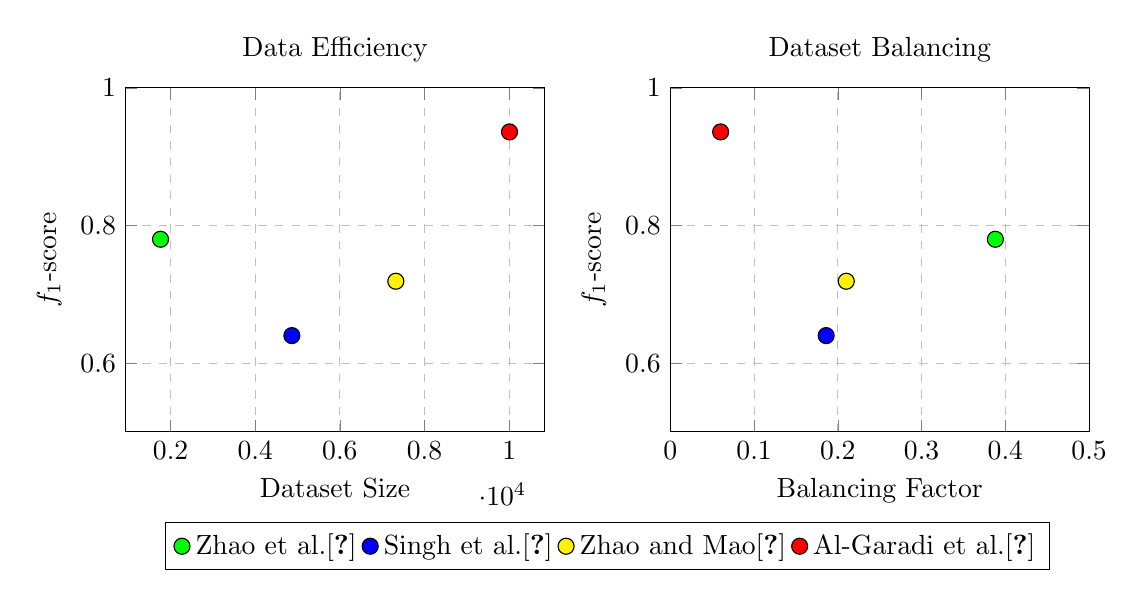
\begin{tikzpicture}
    \begin{groupplot}[group style={
                      group name=datacharts,
                      group size= 2 by 1,
                      horizontal sep=1.6cm}]
        \nextgroupplot[title={Data Efficiency},
                        xlabel={Dataset Size},
                        ylabel={$f_1$-score},
                        ymin=0.5, ymax=1,
                        ymajorgrids=true,
                        xmajorgrids=true,
                        grid style=dashed]
    \addplot[only marks,
            mark=otimes*,
            scatter,
            mark size=2.9pt,
            scatter/classes={
                a={mark=*,green,draw=black},%
                b={mark=*,blue,draw=black},%
                c={mark=*,yellow,draw=black},%
                d={mark=*,red,draw=black}%
            },
            scatter src=explicit symbolic]
    coordinates {
    (1762,0.780) [a]%Zhao et al. (2016)
    %(1954,0.790) %Hosseinmardi et al. (2016)
    %(3279,0.900) %Sugandhi et al. (2016)
    %(4626,0.640) %Dadvar et al. (2013)
    (4865,0.640) [b]%Singh et al. (2016)
    (7321,0.719) [c]%Zhao and Mao (2016)
    (10007,0.936) [d]%Al-Garadi et al. (2016)
    %(13000,0.562) %Zhang et al. (2017)
    %(13160,0.425) %Rosa et al. (2018b)
    %(13160,0.444) %Rosa et al. (2018b)
    };
    \coordinate (c1) at (rel axis cs:0,1);
        \nextgroupplot[title={Dataset Balancing},
                        xlabel={Balancing Factor},
                        ylabel={$f_1$-score},
                        xmin=0, xmax=0.5,
                        ymin=0.5, ymax=1,
                        ymajorgrids=true,
                        xmajorgrids=true,
                        grid style=dashed,
                        legend to name=papers,
                        legend style={legend columns=-1}]
    \addplot[only marks,
            mark=otimes*,
            scatter,
            mark size=2.9pt,
            scatter/classes={
                a={mark=*,green,draw=black},%
                b={mark=*,blue,draw=black},%
                c={mark=*,yellow,draw=black},%
                d={mark=*,red,draw=black}%
            },
            scatter src=explicit symbolic]
    coordinates {
    (0.388,0.780) [a]%Zhao et al. (2016)
    %(1954,0.790) %Hosseinmardi et al. (2016)
    %(0.120,0.900) %Sugandhi et al. (2016)
    %(4626,0.640) %Dadvar et al. (2013)
    (0.186,0.640) [b]%Singh et al. (2016)
    (0.210,0.719) [c]%Zhao and Mao (2016)
    (0.060,0.936) [d]%Al-Garadi et al. (2016)
    %(13000,0.562) %Zhang et al. (2017)
    %(13160,0.425) %Rosa et al. (2018b)
    %(13160,0.444) %Rosa et al. (2018b)
    };
    \coordinate (c2) at (rel axis cs:1,1);
    \legend{Zhao et al.\cite{Zhao2016},Singh et al.\cite{Singh2016},Zhao and Mao\cite{Zhao2017},Al-Garadi et al.\cite{garadi-highestf/top10features}}
    \end{groupplot}
    \coordinate (c3) at ($(c1)!.5!(c2)$);
    \node[below] at (c3 |- current bounding box.south) {\pgfplotslegendfromname{papers}};
\end{tikzpicture}

Analysing the graphs, one can extrapolate that there is direct link between dataset size and set balance, and classifier performance. Models with large amounts of labeled data perform well regardless of balancing, possibly because of a higher probability for that data to sample more edge-cases and therefore extract useful information that would otherwise remain unseen. Surprisingly, the smallest dataset \cite{Zhao2016} performed comparably well, considering it is just $17.61\%$ of the size of the highest performing approach \cite{garadi-highestf/top10features}. This can be attributed to the high balance between the number of cyberbullying and non-cyberbullying instances in the set. Naturally, there is a large difference between the features and techniques used by the reviewed papers, but looking strictly at sizes and balancing, 2 possible approaches become apparent - using either a small but balanced or large and not as balanced dataset. Both could be suitable for this project, since a small set would simulate a scenario for the use of active learning, whereas a large set would allow for a better sampling range while training.

Considering the scope and time constraints of the project, using/compiling a small but balanced dataset seems appropriate.
%%end lit review
%%\newpage
\section{Summary}
\begin{enumerate}
  \item User-based features improve the overall performance of classification, but only marginally.
  \item TF-IDF measure contributes to classification performance most.
  \item Feature engineering is not rewarding.
  \item Choice of machine learning classifier has low impact on performance in most cases.
  \item Naturally probabilistic classification models are better suited for the project's goals.
  \item Pool-Based Sampling is the most applicable scenario for this project.
  \item Small but balanced datasets perform comparably to large unbalanced sets, at a fraction of the data cost.
\end{enumerate}
%%end summary
\section{Design}
\subsection{Specification}
The dataset used for training different machine learning algorithms will be compiled using Twitter's Developer API. As the technique used to collect the data is outside the scope of the project, the open-source library ``Tweepy" will be utilised. It is a Python wrapper for Twitter's API, that removes unnecessary complexity and speeds up the collection process.
A python script will be developed that fetches public tweets based on input keywords. The keywords used when data mining will be chosen based on the probability of the results containing cyberbullying traces. Hence, keywords related to events which often receive negative sentiments, such as celebrities getting ``cancelled", ought to yield more useful data samples than unrelated keywords. However, to obtain a balanced dataset, it is important to also consider keywords not related to bullying, but sentiment or opinion expression in general.
Alongside the tweet's text, the script will parse information about the tweet's author too.

The obtained dataset will then be processed according to the various techniques discussed in section ``Feature Engineering". Notably, textual features will be extracted via natural language processing, while user features will mostly remain raw, as collected by the script. For NLP, open-source libraries like NLTK and openNLP can greatly simplify the task of processing tweets.

To accommodate the sampling process of active learning, a single-page web application will be developed, where the user is interactively queried to label data instances. The tweets displayed will be actively updated by the online active learning process, which orders instances based on some uncertainty measure and stores them in a queue. The user has the ability to skip certain tweets, if they are unsure about correctly labelling them, which displays the next tweet in queue and notes the user's decision.
The view of the application will consist of:
\begin{itemize}
    \item Read-only text box, displaying the tweet's content.
    \item Button for each applicable classification label.
    \item Undo button, that allows the user to review their previous label.
    \item Button for recalculating the uncertainty measures of unlabeled data points.
    \item Real-time dashboard of widgets, containing information regarding the active learning process' state (i.e. number of labels left, estimated classification performance, confidence of the currently displayed tweet, etc.)
\end{itemize}
The application will be built on the MERN stack (MongoDB, Express, React, Node), due to familiarity with the technologies. However, the infrastructure may change, as this is an early design specification. It is possible that a Django/Flask-based application could provide better interoperability with the active learning process, which will be implemented in Python. If so, the specification will be changed accordingly.

For analysis of data efficiency, the following machine learning algorithms will be implemented, as they were found most appropriate during literature review:
\begin{itemize}
    \item Active Learning Logistic Regression
    \item SVM
    \item Logistic Regression
    \item Random Forest
\end{itemize}
Open-source libraries like scikit-learn, NumPy, modAL, libact, etc. will be utilised where possible, as that would save valuable time and therefore enable me to focus on iteratively tuning and improving the system.
If time allows, active learning versions of the SVM and Random Forest algorithms will also be implemented. In such case, the algorithm analysis would greatly benefit from additional information, resulting in more accurate project findings and conclusions.
\subsection{Tasks}
The following tasks need to be completed in order to consider the project successful:
\begin{itemize}
    \item Develop a Twitter crawler - needed for the collection of data from Twitter
    \item Data mining and analysis - collection, preprocessing, feature engineering and selection of dataset obtained as a result of using the Twitter crawler
    \item Develop a web application - front end to the active learning process, interactively queries the user to label data.
    \item Active learning - training of a classification model using active learning
    \item Machine learning (other) - training of classification models using non-active learning techniques
    \item Active learning analysis - review of the findings obtained after applying active learning 
    \item Algorithm comparison - conclusions about data efficiency and visualisation of performance for the explored algorithms
\end{itemize}
Data labeling is performed implicitly throughout the duration of the project.
\subsection{Architecture}
The following diagram outlines the planned structure and general flow of the system:
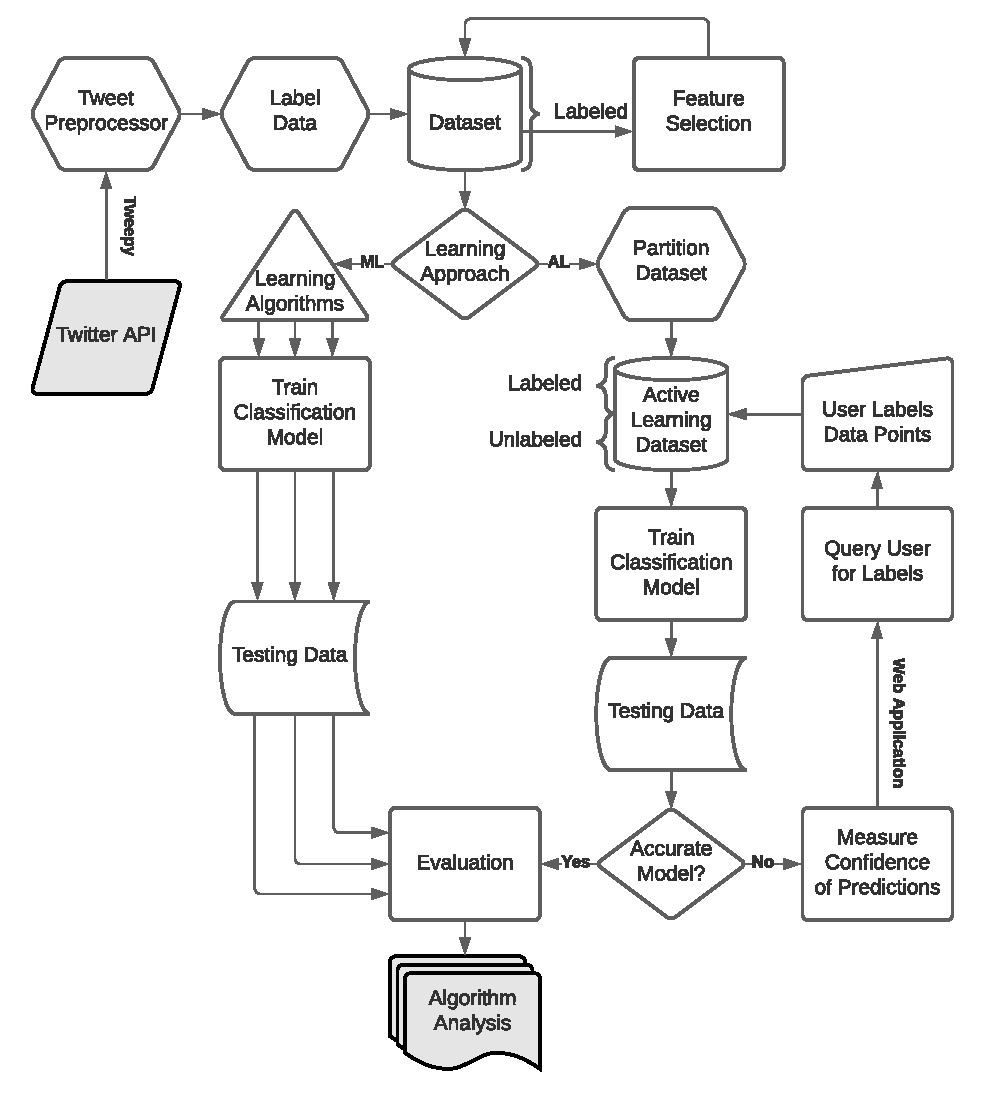
\includegraphics[scale=0.84]{Active Learning.pdf}
\subsection{Evaluation}
Evaluation will be performed by a controlled experiment, where Machine Learning models will be trained with different supervised algorithms but with identical dataset, features and hyperparameters, as well as minimised variance, whenever consistency isn't possible. An exception to this will be the active learning algorithm(s), which to simulate real world application of the technique, will have access to a limited subset of labeled examples, while the rest of the dataset will remain unlabeled.
\subsection{Analysis}
\begin{itemize}
    \item Requirements
    \begin{enumerate}
        \item The dataset must not contain references or links to Twitter users, i.e. complies with privacy laws and guidelines.
        \item All data must be labeled accurately.
        \item The dataset should sample a large enough space, accounting for edge cases whenever possible.
        \item The algorithm should perform well on training and testing data.
        \item Identifying cyberbullying instances correctly (recall) should take precedence over not misclassifying non-bullying instances (precision).
    \end{enumerate}
    \item Costs
    \begin{enumerate}
        \item Monetary investment if data labeling is outsourced to an external party.
        \item Time investment if labeling done independently.
    \end{enumerate}
    \item Benefits
    \begin{enumerate}
        \item Using a single dataset allows for the training of multiple classification models asynchronously.
        \item Data efficiency, low data labeling costs.
        \item Stimulates research in the field of active learning, especially for practical applications.
        \item Minimal variance during evaluation ensures accurate results and findings.
        \item Relatively easy implementation using open-source libraries.
        \item Accelerates startups interested in cyberbullying detection.
    \end{enumerate}
    \item Constraints
    \begin{enumerate}
        \item Limited time restricts the size of the dataset that can be acquired and labeled.
        \item Limited number of data annotators, resulting in lower initial performance.
    \end{enumerate}
    
\end{itemize}
\section{Project Planning}
\subsection{Work Estimate}
 \begin{tabular}{|l l|} 
 \hline
 Task & Time \\ [0.3ex] 
 \hline\hline
 Twitter Crawler & 3 weeks* \\ 
 \hline
 Data Mining & 1 week \\
  \hline
 Data Analysis & 2 weeks \\
 \hline
 Web Application & 2 weeks \\
 \hline
 Active Learning & 2 weeks \\
 \hline
 Other ML Algorithms & 2 weeks \\
 \hline
 Algorithm Refinement & 2 weeks \\
 \hline
 AL Analysis & 2 weeks \\
 \hline
 Algorithm Comparison & 2 weeks \\
 \hline
 Project Refinement & 11 days \\
 \hline
\end{tabular}

*accounts for Christmas and exams
\subsection{Gantt Plots}
\begin{ganttchart}[
        vgrid={*{3}{draw=none},{loosely dotted},
        *{6}{draw=none},{densely dotted},
        *{6}{draw=none},{loosely dotted},
        *{6}{draw=none},{densely dotted},
        *{6}{draw=none},{loosely dotted},
        *{6}{draw=none},{densely dotted},
        *{6}{draw=none},{loosely dotted},
        *{6}{draw=none},{densely dotted},
        *{6}{draw=none},{loosely dotted},
        *{6}{draw=none},{densely dotted},
        *{6}{draw=none},{loosely dotted},
        *{6}{draw=none},{densely dotted},
        *{6}{draw=none},{loosely dotted},
        *{6}{draw=none},{densely dotted},
        *{6}{draw=none},{loosely dotted},
        *{6}{draw=none},{densely dotted},},
        calendar week text=\currentweek ,
        vrule/.style={thick, black},
        x unit=1mm,
        y unit chart=1.5cm,
        time slot format=isodate,
        time slot unit=day,
        bar height = 0.6, %necessary to make it fit the height
        bar top shift = 0.2, %to move it inside the grid space ;)
        newline shortcut=true,
        bar label node/.append style=%
        {align=left,text width={width("Specification ")}},
        Mile1/.style={milestone/.append style={fill=red, shape=circle,scale=0.5}},
        milestone label font=\normalsize
        ]{2020-10-01}{2021-01-17}
        \gantttitlecalendar{year, month=shortname, week=1} \\
        \ganttbar{Background\\Reading}{2020-10-01}{2020-12-08}] \\
        \ganttbar{Literature\\Review}{2020-10-17}{2020-11-15}] \\
        \ganttbar{Design\\Specification}{2020-11-16}{2020-11-30}] \\
        \ganttbar{Project\\Planning}{2020-12-01}{2020-12-08}] \\
        \ganttbar{Twitter\\Crawler}{2020-12-16}{2021-01-10}]
        \ganttvrule{Project Brief}{2020-10-16}
        \ganttvrule{Progress Report}{2020-12-08}
\end{ganttchart}
    
\begin{ganttchart}[
        vgrid={*{6}{draw=none},{loosely dotted},
               *{6}{draw=none},{densely dotted}},
        calendar week text=\currentweek ,
        vrule/.style={thick, black},
        vrule label node/.append style={anchor=north east},
        x unit=1mm,
        y unit chart=1.5cm,
        time slot format=isodate,
        time slot unit=day,
        bar height = 0.6, %necessary to make it fit the height
        bar top shift = 0.2, %to move it inside the grid space ;)
        newline shortcut=true,
        bar label node/.append style=%
            {align=left,text width={width("Comparison ")}},
        group label node/.append style=%
            {align=left,text width={width("Comparison ")}}
        ]{2021-01-04}{2021-04-30}
        \gantttitlecalendar{year, month=shortname, week=16} \\
        \ganttbar{Data\\Mining}{2021-01-11}{2021-01-17}] \\
        \ganttbar{Web\\Application}{2021-01-11}{2021-01-28}] \\
        \ganttbar{Data\\Analysis}{2021-01-18}{2021-01-31}] \\
        \ganttgroup{Algorithm\\Design}{2021-02-01}{2021-03-14} \\
        \ganttbar{Active\\Learning}{2021-02-01}{2021-02-14}] \\
        \ganttbar{Other ML\\Algorithms}{2021-02-15}{2021-02-28}] \\
        \ganttbar{Algorithm\\Refinement}{2021-02-29}{2021-03-14}] \\
        \ganttgroup{Evaluation}{2021-03-15}{2021-04-15} \\
        \ganttbar{AL\\Analysis}{2021-03-15}{2021-03-31}] \\
        \ganttbar{Algorithm\\Comparison}{2021-04-01}{2021-04-15}] \\
        \ganttbar{Project\\Refinement}{2021-04-16}{2021-04-27}]
        \ganttvrule{Project Report}{2021-04-27}
\end{ganttchart}
\newpage
\subsection{Iterations}
The project has been split into tasks that take approximately a week to prototype or implement. However, two weeks have been allocated per task, as this allows for phased iterative development, where deliverables go through refinement individually. That is, after each component is completed, there is a period of time reserved for the sole purpose of improving the design and implementation, before moving on to the next one. As deliverables depend on the success of their predecessor, this approach ensures the project is always moving forward smoothly. The time that remains after finishing all listed tasks will be utilised for a final iteration of the system as a whole.
\subsection{Tools}
The following tools will be utilised as a means of speeding up the development process, scheduling, keeping track of progress and report writing:

\begin{tabular}{|l l l|} 
 \hline
 Tool & Description & Benefit \\ [0.3ex] 
 \hline\hline
 Git & Version Control & Tracking of changes during development \\ 
 \hline
 Mendeley & Reference Manager & Collection of research papers and citations \\
  \hline
 Notion & Notes \& Workflow & Project management and progress tracking \\
 \hline
 ECS GPU & Compute Service & High availability, efficient machine learning \\
 \hline
 Overleaf & LaTeX Editor & Project report sync between devices \\
 \hline
 Lucidchart & Charts \& Diagrams & Design sketching and visualisation \\
 \hline
\end{tabular}
\subsection{Risk Assessment}
\begin{tabular}{|l|l|l|}
\hline
\multicolumn{3}{|l|}{\parbox[t]{\textwidth-1.15cm}{\textbf{PROBLEM}: Lack of experience with machine learning technologies}} \\ \hline
\textbf{LOSS}: 3& \textbf{PROBABILITY}: 2&\textbf{RISK}: 6\\ \hline
\multicolumn{3}{|l|}{\parbox[t]{\textwidth-1.15cm}{\textbf{PLAN}: Enrolled in two machine learning related modules throughout the academic year, which alongside personal reading and experimentation should provide the necessary background to implement this project.}} \\ \hline
\end{tabular}

\begin{tabular}{|l|l|l|}
\hline
\multicolumn{3}{|l|}{\parbox[t]{\textwidth-1.15cm}{\textbf{PROBLEM}: Overambitious deliverables - unable to finish task in the planned time frame\vspace{.2\baselineskip}}} \\ \hline
\textbf{LOSS}: 4& \textbf{PROBABILITY}: 2&\textbf{RISK}: 8\\ \hline
\multicolumn{3}{|l|}{\parbox[t]{\textwidth-1.15cm}{\textbf{PLAN}: The iterative approach discussed earlier allows for up to a week of time after the initial completion of a task and is used for refinement. However, if necessary, this time can be reallocated to completing the problematic task and skipping the iterative process with no significant consequences. This generally shouldn't happen as work is scheduled according to personal capabilities.}} \\ \hline
\end{tabular}

\begin{tabular}{|l|l|l|}
\hline
\multicolumn{3}{|l|}{\parbox[t]{\textwidth-1.15cm}{\textbf{PROBLEM}: Data labeling takes too much time, staggered progress and productivity\vspace{.2\baselineskip}}} \\ \hline
\textbf{LOSS}: 5& \textbf{PROBABILITY}: 3&\textbf{RISK}: 15\\ \hline
\multicolumn{3}{|l|}{\parbox[t]{\textwidth-1.15cm}{\textbf{PLAN}: Data labeling will be outsourced to external party if necessary or the planned dataset size will be reduced to accommodate the loss of time.}} \\ \hline
\end{tabular}

\begin{tabular}{|l|l|l|}
\hline
\multicolumn{3}{|l|}{\parbox[t]{\textwidth-1.15cm}{\textbf{PROBLEM}: Illness or otherwise reduced ability to work}} \\ \hline
\textbf{LOSS}:2 & \textbf{PROBABILITY}: 2&\textbf{RISK}: 4\\ \hline
\multicolumn{3}{|l|}{\parbox[t]{\textwidth-1.15cm}{\textbf{PLAN}: Similar to the risk of overambitious deliverables, time that would usually be spent refining completed tasks can be reallocated for emergencies with no major setbacks.}} \\ \hline
\end{tabular}
%%\newpage
%%end planning
\bibliographystyle{ieeetr}
\bibliography{library.bib}
\end{document}